\subsection{Mapping $\mathcal{F}$ to $2$-adic integers} \label{subsec:2-adics}

Let $\mathcal{F}$ denote the set of functions $f: \mathbb{Z}_{\geq 0}\to\mathbb{Z}$ such that $2^n\mid (\Delta^nf)(x)$ for all $n\geq 0$ and $x\in \mathbb{Z}_{\geq 0}$. Define the shift operator $S$ by
\[(Sf)(x)=f(x+1).\]

\begin{lemma}
\label{lem:productrule}
The product rule
\[\Delta^n(f\cdot g)=\sum_{k=0}^{n}\binom{n}{k}\Delta^{n-k}\left(S^k(f)\right)\Delta^k(g)\]
holds, which can be extended to multiple functions as
\[\Delta^n(f_1\dotsm f_m)=\sum_{a_1+\dotsb+a_m=n}\binom{n}{a_1, \dotsc, a_m}\Delta^{a_1}(S^{a_2+\dotsb+a_m}f_1)\cdot \Delta^{a_2}(S^{a_3+\dotsb+a_m}f_2)\dotsm \Delta^{a_m}(f_m).\]
\end{lemma}

\begin{lemma}
\label{lem:F closure}
The set $\mathcal{F}$ is closed under the following operations:
\[f\mapsto Sf, \quad (f, g)\mapsto f\cdot g, \quad \text{ and }\quad (f, g)\mapsto \langle f, g\rangle = \frac{f(x+1)g(x)+f(x)g(x+1)}{2}.\]
\end{lemma}
\begin{proof}
    Closure under $S$ is clear. For multiplication, we may use the product rule: each individual term in the expansion of $\Delta^n(f\cdot g)$ will be divisible by $2^n$. Likewise, by writing
    \[\langle f, g\rangle = f\cdot g + \frac{\Delta(f)\cdot g+f\cdot \Delta(g)}{2}\]
    and expanding with the product rule, we can show that $\langle f, g\rangle\in\mathcal{F}$ if $f, g\in\mathcal{F}$.
\end{proof}

Next, observe that for $f\in \mathcal{F}$ and any nonnegative integer $n$, we have $(\Delta^nf)(x)\equiv 0\pmod{2^n}$ by definition and also $(\Delta^{n+1}f)(x)\equiv 0\pmod{2^{n+1}}$. Then $\Delta^nf$ is constant modulo $2^{n+1}$ and must be equal to either $2^{n}$ or $0$. Define a mapping
\[\varepsilon: \mathcal{F}\to\{0, 1\}^{\mathbb{N}}\]
by sending $f$ to $(\varepsilon_0^f, \varepsilon_1^f, \dotsc)$ where 
\[
\varepsilon_n^f=\begin{cases}
0 & \text{ if }\Delta^nf\equiv 0\pmod {2^{n+1}} \\
1 & \text{ if }\Delta^nf\equiv 2^n\pmod{2^{n+1}}
\end{cases}.
\]

Define the weight of a binary tree $T$ by
\[w_b(T; x)=\prod_{v\in T}b(x+l_v)\]
where the product is over all vertices $v$ of $T$ and $l_v$ the number of left-edges in the path from the root to $v$. Evaluating this weight at $x=0$ and summing over all binary trees gives $C^b_n$. For each orbit $\mathcal{O}$, define a total weight function $w_{\mathcal{O}}(x)$ by
\[w_{\mathcal{O}}(x)=\sum_{T\in\mathcal{O}}w_b(T)\]
and the average weight function $r_b(\mathcal{O}; x)$ by
\[r_b(\mathcal{O}; x)=\frac{w_b(\mathcal{O}; x)}{\lvert\mathcal{O}\rvert}.\]
We have the recursive formula
\[r_b(\mathcal{O}; x)=b(x)\cdot\langle r_b(\mathcal{O}_L; x), r_b(\mathcal{O}_R; x)\rangle\]
(see Postnikov and Sagan \cite{postnikov2007power}) where $\mathcal{O}_L$ and $\mathcal{O}_R$ are the orbits associated to the left and right subtrees of the root. By Lemma \ref{lem:F closure} and induction, all functions $r_b(\mathcal{O}; x)$ are in $\mathcal{F}$.

\begin{definition}\label{def:epsilonO}
For an orbit $\mathcal{O}$ of binary trees, let $\varepsilon^{\mathcal{O}}_m=\varepsilon^f_m$ for $f=r_b(\O)\in \mathcal{F}$.
\end{definition}

From now on, we will also let $\varepsilon_k=\varepsilon^b_k$ for all $k$, i.e. the superscript $b$ will be omitted.

\begin{lemma}
\label{lem:epsilon formula}
For an orbit $\mathcal{O}$ with left and right orbits $\mathcal{O}_L, \mathcal{O}_R$, the following formula holds:
\[\varepsilon^{\mathcal{O}}_{m} \equiv\sum_{i+j+k=m}\binom{m}{i, j, k}\varepsilon_{k}(\varepsilon^{\mathcal{O}_L}_{i}\varepsilon^{\mathcal{O}_R}_j+\varepsilon^{\mathcal{O}_L}_{i+1}\varepsilon^{\mathcal{O}_R}_j+\varepsilon^{\mathcal{O}_L}_{i}\varepsilon^{\mathcal{O}_R}_{j+1})\pmod{2}.\]
\end{lemma}
\begin{proof}
    We make use of the identity 
    \[\langle f, g\rangle = f\cdot g + \frac{\Delta(f)\cdot g+f\cdot \Delta(g)}{2}.\]
    By expanding with the product rule, we have
    \begin{align*}
        \Delta^mr_b(\mathcal{O}; x)=\sum_{i+j+k=m} &\binom{m}{i, j, k}\Big[\Delta^k(S^{i+j}b)\cdot\Big(\Delta^{i}(S^jr_b(\mathcal{O}_L; x))\cdot \Delta^j(r_b(\mathcal{O}_R; x))+ \\
        &\frac{\Delta^{i+1}(S^jr_b(\mathcal{O}_L; x))\cdot \Delta^j(r_b(\mathcal{O}_R; x))+\Delta^{i}(S^jr_b(\mathcal{O}_L; x))\cdot \Delta^{j+1}(r_b(\mathcal{O}_R; x))}{2}\Big)\Big].
    \end{align*}
    We may now break this up into three sums, each of which will correspond to a term in the statement in the lemma. The first term is
    \[\sum_{i+j+k=m}\binom{m}{i, j, k}\Delta^k(S^{i+j}b)\cdot\Delta^{i}(S^jr_b(\mathcal{O}_L; x))\cdot \Delta^j(r_b(\mathcal{O}_R; x))\]
    As $b, r_b(\mathcal{O}_L; x), r_b(\mathcal{O}_R; x)\in \mathcal{F}$, each term in this summation is divisible by $2^k\cdot 2^i\cdot 2^j=2^m$. This term is \emph{not} divisible by $2^{m+1}$ if and only if all of the following hold:
    \begin{itemize}
        \item $\binom{m}{i, j, k}$ is odd.
        \item $\Delta^k(S^{i+j}b)\equiv 2^k\pmod{2^{k+1}}$.
        \item $\Delta^i(S^jr_b(\mathcal{O}_L; x))\equiv 2^i\pmod{2^{i+1}}$.
        \item $\Delta^{j}(r_b(\mathcal{O}_R; x))\equiv 2^j\pmod{2^{j+1}}$.
    \end{itemize}
    Therefore the residue modulo $2^{m+1}$ is equal to the residue of
    \[\sum_{i+j+k=m}\binom{m}{i, j, k}\varepsilon_k\varepsilon^{\mathcal{O}_L}_i\varepsilon^{\mathcal{O}_R}_{j}\]
    modulo $2$, multiplied by $2^m$.
    
    Similarly, the second term in the expansion is
    \[\frac{1}{2}\sum_{i+j+k=m}\binom{m}{i, j, k}\Delta^k(S^{i+j}b)\cdot\Delta^{i+1}(S^jr_b(\mathcal{O}_L; x))\cdot \Delta^j(r_b(\mathcal{O}_R; x)).\]
    The summation without the factor of $\frac{1}{2}$ is always a multiple of $2^{m+1}$, and will not be a multiple of $2^{m+2}$ if and only if $\binom{m}{i, j, k}$ is odd and $\varepsilon^b_k=\varepsilon^{\mathcal{O}_L}_{i+1}=\varepsilon^{\mathcal{O}_R}_{j}=1$. The third term can be handled similarly. Summing all the equations yields the lemma.
    
    In the case where $\mathcal{O}_L$ or $\mathcal{O}_R$ is empty, the associated function is $r_b=1$ with $\varepsilon^{r_b}_0=1$ and $\varepsilon^{r_b}_k=0$ for $k\geq 1$. The proof of the lemma works the same in this case.
\end{proof}

\begin{lemma}
    \label{lem:reduction}
    Let $\mathcal{O}$ be an orbit of binary trees on $n$ vertices, and suppose that for some vertex $v$, the subtree with root $v$ is a complete binary tree of depth $k$. Let $\mathcal{O}'$ be the same orbit of trees with the subtree at $v$ replaced by a single vertex at $v$. Then \[\varepsilon_m^{\mathcal{O}}=\varepsilon_0^{2^k-2}\varepsilon_m^{\mathcal{O}'}.\]
\end{lemma}

\begin{proof}
    We prove this lemma by induction. If $v$ is not the root vertex, then we use lemma \ref{lem:epsilon formula} to expand. Exactly one of the left and right subtrees contains $v$, so the inductive hypothesis applies to factor out $\varepsilon_0^{2^k-2}$. Hence we can reduce to the base case where $v$ is the root, i.e. we have a complete binary tree of depth $k$. To prove this case, we induct on $k$.
    
    For $k=1$ the lemma follows because $r_b(\mathcal{O}; x)=b(x)$. For the inductive step, we use Lemma \ref{lem:epsilon formula} where $\mathcal{O}_L$ and $\mathcal{O}_R$ are complete binary trees of depth $k-1$. Note that by symmetry of $i$ and $j$, the $\varepsilon^{\mathcal{O}_L}_{i+1}\varepsilon^{\mathcal{O}_R}_j+\varepsilon^{\mathcal{O}_L}_{i}\varepsilon^{\mathcal{O}_R}_{j+1}$ term cancels out in the sum, and $\varepsilon^{\mathcal{O}_L}_{i}\varepsilon^{\mathcal{O}_R}_j$ also cancels out for all terms where $i\neq j$. Finally, note that if $i=j > 0$, then the binomial coefficient $\binom{m}{i, j, k}=\binom{m}{k}\binom{i+j}{i}$ is divisible by $\binom{2i}{i}$, which is even. Therefore the only remaining term in the summation is the $i=j=0$ term. By the inductive hypothesis, we have
    \[\varepsilon^{\mathcal{O}}_m\equiv \varepsilon_m^{\mathcal{O'}}\varepsilon_0^{2(2^{k-1}-1)}=\varepsilon_0^{2^k-2}\varepsilon_m^{\mathcal{O}'}\]
    as desired.
\end{proof}

The recursive formula illustrated in Lemma~\ref{lem:epsilon formula} enables us to explicitly write down $\varepsilon_m^{\O}$ in an elegant way. This combinatorial description gives another quick proof to Lemma~\ref{lem:reduction} but is not used in other places of the paper. Readers are free to skip to the proof of the main theorem.

We view an orbit $\O$ as a rooted binary tree. Traditionally, we say that a vertex $v$ is a descendant of another vertex $w$ in $\O$ if the unique path connecting $v$ and the root passes through $w$. Similarly, we say that a vertex $v$ is a \textit{descendant} of an edge $e$ in $\O$ if the unique path connecting $v$ and the root contains $e$. In addition, we say that an edge $e$ of $\O$ connecting two vertices $u$ and $v$ \textit{originates from} $u$ if $v$ is a descendant of $e$ (or of $u$). Consequently, two edges $e$ and $e'$ are called \textit{siblings} if they originate from the same vertex.
\begin{definition}\label{def:coin}
A \textit{coin-configuration} $C$ on $\O$ of order $m$ consists of the following data:
\begin{itemize}
    \item a subset of edges $E$ of $\O$ such that no siblings are simultaneously selected,
    \item a distribution of distinct \textit{coins} $\{1,\ldots,m\}\cup E$ to all vertices of $\O$ such that each coin $c_e$ labeled by an edge $e\in E$ is assigned to a descendent of $e$.
\end{itemize}
For such a coin-configuration $C$, let $C_v$ denote the set of coins at $v$. Define its weight $\wt(C)=\prod_{v\in\O}\varepsilon_{|C_v|}$ where the product is over all vertices $v$ in $\O$. Moreover, let $\mathcal{C}^{\O}_m$ denote the set of all coin-configurations on $\O$ of order $m$. 
\end{definition}
See Figure~\ref{fig:coin} for an example of a coin-configuration of order 9 on an orbit $\O$ which is a rooted binary tree on 8 vertices, where the selected edges in $E$ are highlighted as thick line segments and the distribution of coins is written underneath the vertices. This particular example has weight $(\varepsilon_0)^2(\varepsilon_1)(\varepsilon_2)^4(\varepsilon_3)$.
\begin{figure}[h!]
\centering
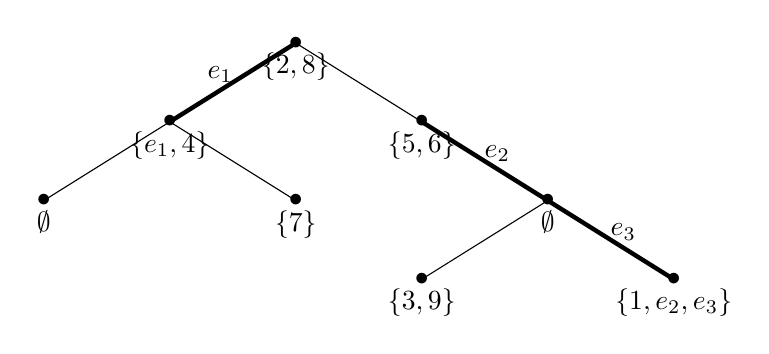
\begin{tikzpicture}[x=1.6cm]
\node at (0,0) {$\bullet$};
\node[below] at (0,0) {$\{2,8\}$};
\node at (-1,-1) {$\bullet$};
\node[below] at (-1,-1) {$\{e_1,4\}$};
\node at (-2,-2) {$\bullet$};
\node[below] at (-2,-2) {$\emptyset$};
\node at (0,-2) {$\bullet$};
\node[below] at (0,-2) {$\{7\}$};
\node at (1,-1) {$\bullet$};
\node[below] at (1,-1) {$\{5,6\}$};
\node at (2,-2) {$\bullet$};
\node[below] at (2,-2) {$\emptyset$};
\node at (3,-3) {$\bullet$};
\node[below] at (3,-3) {$\{1,e_2,e_3\}$};
\node at (1,-3) {$\bullet$};
\node[below] at (1,-3) {$\{3,9\}$};
\draw (-2,-2)--(-1,-1)--(0,0)--(1,-1)--(2,-2)--(3,-3);
\draw (0,-2)--(-1,-1);
\draw (2,-2)--(1,-3);
\draw[ultra thick] (0,0)--(-1,-1);
\draw[ultra thick] (1,-1)--(2,-2);
\draw[ultra thick] (2,-2)--(3,-3);
\node at (-0.6,-0.4) {$e_1$};
\node at (1.6,-1.4) {$e_2$};
\node at (2.6,-2.4) {$e_3$};
\end{tikzpicture}
\caption{An example of a coin-configuration of order 9 with weight $(\varepsilon_0)^2(\varepsilon_1)(\varepsilon_2)^4(\varepsilon_3)$.}
\label{fig:coin}
\end{figure}

\begin{proposition}\label{prop:coin}
We have the following explicit formula for an orbit $\O$:
$$\varepsilon_m^{\O}=\sum_{C\in\mathcal{C}^{\O}_m}\wt(C)$$
where the sum is over all coin-configurations $C$ on $\O$ of order $m$.
\end{proposition}
\begin{proof}
The proposition is a direct consequence of Lemma~\ref{lem:epsilon formula} and induction on the number of vertices of $\O$. For the base case where $\O$ is a single vertex, by definition, $\varepsilon^{\O}_m$ equals $\varepsilon_m$. At the same time, we have exactly 1 coin-configuration with weight $\varepsilon_m$ since there are no edges and all $m$ coins must be assigned to the unique vertex in $\O$.

Now assume that our proposition is true for all orbits with less than $n$ vertices and consider an orbit $\O$ with $n$ vertices. Similarly as in Lemma~\ref{lem:epsilon formula}, let $\O_L$ and $\O_R$ be the left and right subtrees of the root respectively and let $e_L$ and $e_R$ be the left and right edges originating from the root respectively. Consider $\sum_{C\in\mathcal{C}^{\O}_m}\wt(C)$, which is the RHS of the proposition. For a coin-configuration $C$ with a chosen subset $E$ of the edges, we cannot have both $e_L$ and $e_R$ lie in $E$. Then there are 3 possibilities: (1) $e_L\in E$, $e_R\notin E$; (2) $e_L\notin E$, $e_R\in E$; (3) $e_L,e_R\notin E$. For (1), we have $\binom{m}{i,j,k}$ ways to assign $k$ coins to the root, $i+1$ total coins to the left subtree ($i$ original coins in $\{1,\ldots,m\}$ and a new coin from $e_L$), and $j$ total coins to the right subtree. This provides a sum of $$\sum_{i+j+k=m}\binom{m} {i,j,k}\varepsilon_k\sum_{C\in\mathcal{C}^{\O_L}_{i+1}}\wt(C)\sum_{C\in\mathcal{C}^{\O_R}_{j}}\wt(C)=\sum_{i+j+k=m}\binom{m} {i,j,k}\varepsilon_k\varepsilon_{i+1}^{\O_L}\varepsilon_{j}^{\O_R}$$
by induction. Similarly handle case (2) and (3) and take the total sum $\sum_{C\in\mathcal{C}^{\O}_m}\wt(C)$, which is the exact same expression as RHS of Lemma~\ref{lem:epsilon formula} so it equals $\varepsilon_m^{\O}$ as desired.
\end{proof}

From the description of $\varepsilon_m^{\O}$ using coin-configurations (Definition~\ref{def:coin}), Lemma~\ref{lem:reduction} becomes immediate: if a vertex $v$ of $\O$ has isomorphic left and right subtrees, we can pair up coin-configurations with nontrivial coin assignments to descendents of $v$ by switching the left and right subtrees of $v$ and each pair of coin-configurations have the same weight.